\documentclass[compress]{beamer}        % [compress] (written before {beamer} <=> navigation bar one line, all subsections in 1 line instead of 2

% Setup appearance:
\usetheme{CambridgeUS}
%	AnnArbor | Antibes | Bergen |
%	Berkeley | Berlin | Boadilla |
%	boxes | CambridgeUS | Copenhagen |
%	Darmstadt | default | Dresden |
%	Frankfurt | Goettingen |Hannover |
%	Ilmenau | JuanLesPins | Luebeck |
%	Madrid | Malmoe | Marburg |
%	Montpellier | PaloAlto | Pittsburgh |
%	Rochester | Singapore | Szeged |
%	Warsaw
%

\useoutertheme[footline=authorinstitute,subsection=false]{miniframes}
\usecolortheme{whale}

%	albatross | beaver | beetle |
%	crane | default | dolphin |
%	dove | fly | lily | orchid |
%	rose |seagull | seahorse |
%	sidebartab | structure |
%	whale | wolverine


\setbeamertemplate{footline}
{
  \hbox{%
  \begin{beamercolorbox}[wd=.25\paperwidth,ht=2.25ex,dp=1ex,center]{title in head/foot}%
    \usebeamerfont{date in head/foot}\insertshortauthor
  \end{beamercolorbox}%
  \begin{beamercolorbox}[wd=.5\paperwidth,ht=2.25ex,dp=1ex,center]{date in head/foot}%
    \usebeamerfont{title in head/foot}\insertshortinstitute
  \end{beamercolorbox}%
  \begin{beamercolorbox}[wd=.25\paperwidth,ht=2.25ex,dp=1ex,center]{title in head/foot}%
    \usebeamerfont{date in head/foot}
    \insertframenumber{} / \inserttotalframenumber
    %\insertframenumber{} / \insertpresentationendpage
  \end{beamercolorbox}}%
  \vskip0pt%
}

%\setbeamercolor{titlelike}{parent=structure}
%\setbeamercolor{structure}{fg=beamer@blendedblue}
%% \useinnertheme{rounded}
%\setbeamerfont{block title}{size={}}
%\usefonttheme[onlylarge]{structurebold}   % title and words in the table of contents bold
%\setbeamerfont*{frametitle}{size=\normalsize,series=\bfseries}
\setbeamertemplate{navigation symbols}{}
\setbeamercolor{frametitle}{parent=boxes, bg=white}
{ % only on titlepage


\usepackage{times}
\usepackage{amsmath,amssymb,amsthm}
\usepackage{color}
\usepackage{changepage}
\usepackage{multirow}
\usepackage[absolute,overlay]{textpos}
\usepackage{enumerate}
%\usepackage{pgfpages}
\usepackage[all]{xy}
\usepackage{textcomp}
\usepackage{etex}
\usepackage{tikz}
\usetikzlibrary{shapes}
%\usepackage{handoutWithNotes}
%\pgfpagesuselayout{4 on 1}[border shrink=1mm]




\definecolor{camblue}{RGB}{26,26,89}
\definecolor{Rblue}{RGB}{0,255,255}
\definecolor{Rdarkblue}{RGB}{0,0,255}
\definecolor{Rgreen}{RGB}{0,205,0}
\definecolor{green2}{RGB}{51,204,51}
\newcommand{\tcb}{\textcolor{beamer@blendedblue}}
\newcommand{\tcbb}{\textcolor{camblue}}
\newcommand{\tcr}{\textcolor{red}}
\newcommand{\tcg}{\textcolor{gray}}
\newcommand{\tcgr}{\textcolor{green2}}
\newcommand{\tcblk}{\textcolor{black}}
\newcommand{\tcRg}{\textcolor{Rgreen}}
\newcommand{\tcRdb}{\textcolor{Rdarkblue}}
\newcommand{\tcRb}{\textcolor{Rblue}}
\newcommand{\tcw}{\textcolor{white}}
\newcommand{\m}{\phantom{-}}
\newcommand{\bp}{\tcbb{$\bullet$}\:}


\title{{\huge Statistics for Computing\\[0.1cm]MA4413}}
\author[Kevin Burke]{{\bf\\[0.5cm]{\huge Lecture 15}\\[0.2cm]\emph{Hypothesis Testing}\\[1.4cm]Kevin Burke}\\[0.3cm]\tcb{kevin.burke@ul.ie}}

\institute[University of Limerick, Maths \& Stats Dept]{}
\date{}

%\TPGrid[5mm,5mm]{1}{1}

\begin{document}


\begin{frame}[t]
\titlepage
\end{frame}



\section{Confidence Intervals}
\subsection{Confidence Intervals}
\begin{frame}{\bf \tcb{Confidence Intervals}}

Confidence intervals are used mainly for \emph{statistical estimation}.\\[0.7cm]

They provide a \emph{range of plausible values} for the parameter of interest at a given level of \emph{confidence} via \\[-0.2cm]
\begin{align*}
\text{statistic} \,\, \pm \,\, z_{\,\alpha/2} \, \times \, s(\text{statistic})\\[-0.2cm]
\end{align*}
where $s(\text{statistic})$ is the \emph{standard error} of the estimate and $z_{\,\alpha/2}$ is the $z$ value which puts probability $\alpha/2$ in the lower and upper tails, i.e.,\\[-0.2cm]
\begin{align*}
\Pr(\text{interval contains parameter}) = 1 - \alpha.\\[-0.3cm]
\end{align*}
$\Rightarrow$ $(1 - \alpha)100\%$ confident that the interval contains the parameter.

\end{frame}





\subsection{Confidence Intervals}
\begin{frame}{\bf \tcb{Confidence Intervals}}

We have calculated confidence intervals for the following parameters:\\[0.1cm]
\begin{itemize}\itemsep0.3cm
\item One mean: $\mu$.
\item One proportion: $p$.
\item Difference between means: $\mu_1 - \mu_2$.
\item Difference between proportions: $p_1 - p_2$.\\[0.3cm]
\end{itemize}

In each case there is a formula for calculating the standard error.\\[0.4cm]

For numerical data, we replace the $z_{\,\alpha/2}$ value with a $t_{\,\nu,\,\alpha/2}$ value when the sample size is small and \emph{approximately normal}.\\[0.4cm]

Furthermore, when comparing means in two small samples, there is a different formula for $s(\,\overline{\!X}_1-\,\overline{\!X}_2)$ if we assume equal variances.


\end{frame}









\subsection{Confidence Intervals for Hypothesis Testing}
\begin{frame}{\bf \tcb{Confidence Intervals for Hypothesis Testing}}

A {\bf hypothesis} is a \emph{belief} about the value of a parameter.\\[0.9cm]

We can use confidence intervals to investigate hypotheses.\\[0.9cm]

Recall the gameplay example from Lecture13 where a developer believes there are 16 hours of gameplay; the \emph{hypothesis} is $\mu = 16$.\\[0.1cm]
\begin{itemize}\itemsep0.4cm
\item Data was collected and a 95\% confidence interval was then calculated: $[14.62, 16.18]$.
\item The interval contains $\mu=16$ and, therefore, we \emph{accept} the hypothesis that there are 16 hours of gameplay.
\end{itemize}
\end{frame}







\section{Hypothesis Testing}
\subsection{Hypothesis Testing}
\begin{frame}{\bf \tcb{Hypothesis Testing}}

There is a more \emph{formal approach} to {\bf hypothesis testing}:

\begin{enumerate}[1.]\itemsep0.3cm
\item State hypotheses \emph{before} collecting data.\\
    \begin{itemize}\itemsep0.2cm
    \item The {\bf null hypothesis}, denoted {\boldmath$H_0$}, is the hypothesis to be tested.
    \item The {\bf alternative hypothesis}, denoted {\boldmath$H_a$}, is the counter-hypothesis, i.e., the \emph{complement} of $H_0$.
    \end{itemize}
\item Choose the {\bf significance level}: the probability of \emph{error} (denoted {\boldmath$\alpha$}) in rejecting $H_0$, i.e., the chance of rejecting $H_0$ when it is true.
\item Collect data and calculate a {\bf test statistic}.
\item Compare this statistic to a {\bf critical value} from statistical tables.
\item Make a decision; either there is:\\
    \begin{enumerate}[a)]\itemsep0.2cm
    \item \emph{Evidence} to {\bf reject} {\boldmath$H_0$} (in favour of $H_a$) at the $\alpha$ significance level.
    \item \emph{Not enough evidence} to reject $H_0$ at the $\alpha$ level, i.e., {\bf accept} {\boldmath$H_0$}.
    \end{enumerate}
\end{enumerate}


\end{frame}



\subsection{Test Statistic}
\begin{frame}{\bf \tcb{Test Statistic}}

By the central limit theorem,
\begin{align*}
\,\overline{\!X} \sim \text{Normal}\left(\mu,\frac{\sigma}{\sqrt{n}}\right) \end{align*}
$\Rightarrow 95\%$  of the time, the $\bar x$  calculated will be in $\mu \pm 1.96\,\frac{\sigma}{\sqrt{n}}$.\\[0.8cm]
Standardising the above gives:
\begin{align*}
Z = \frac{\,\overline{\!X}-\mu}{\sigma / \sqrt{n}} &\sim \text{Normal}\left(0,1\right)
\end{align*}
$\Rightarrow 95\%$  of the time, the {\boldmath$z$} {\bf score} calculated will be in $\pm 1.96$.\\[0.7cm]

{\footnotesize(note: usually $\sigma$ is unknown but when $n > 30$ we can substitute with $s$)}

\end{frame}


\subsection{Test Statistic}
\begin{frame}{\bf \tcb{Test Statistic}}

We \emph{hypothesise} that the true mean is equal to some value, $\mu_0$. This gives us the following null and alternative hypotheses:
\begin{center}
\begin{tabular}{|c@{\,\,}c|}
\hline
&\\[-0.4cm]
$H_0: \quad \mu$ & $= \mu_0$ \\[0.2cm]
$H_a: \quad \mu$ &  $\ne \mu_0$ \\[0.1cm]
\hline
\end{tabular}
\end{center}

Assuming the null hypothesis is true (i.e., $\mu = \mu_0$), we know that, 95\% of the time, the calculated {\bf test statistic}
\begin{align*}
\boxed{z = \frac{\bar x -\mu_0}{s / \sqrt{n}}}
\end{align*}
will be within $\pm 1.96$, i.e., only 5\% of the time will we get a $z$ value outside of this range.

\end{frame}



\subsection{Critical Values}
\begin{frame}{\bf \tcb{Critical Values}}

If our calculated $z$ value is outside of $\pm 1.96$ then we {\bf reject} {\boldmath$H_0$} {\bf at the 5\% level of significance}\,\, {\footnotesize(note: in 5\% of cases we will \emph{wrongly reject} $H_0$)}.\\[1cm]

Of course, we can test $H_0$ at other significance levels by using different {\bf critical values}, $cv$, i.e., the values\\[-0.3cm]
\begin{align*}
\boxed{\pm z_{\,\alpha/2}}\\[-0.3cm]
\end{align*}
correspond to testing at the $\alpha$ significance level and, furthermore, if $n\le30$, the critical values come from the t tables:\\[-0.3cm]
\begin{align*}
\boxed{\pm t_{\,\nu,\,\alpha/2}}.
\end{align*}

\end{frame}



\subsection{Hypothesis Testing Procedure}
\begin{frame}{\bf \tcb{Hypothesis Testing Procedure}}

\begin{enumerate}[1.]\itemsep0.4cm
\item When testing the hypothesis that $\mu = \mu_0$ we have:\\
    \begin{itemize}\itemsep0.3cm
    \item $H_0:$ $\mu = \mu_0$,
    \item $H_a:$ $\mu \ne \mu_0$.
    \end{itemize}
\item Select the $\alpha$ level, e.g., $\alpha = 0.05$.
\item Collect data $\Rightarrow$ calculate $\bar x$, $s$ and, hence, the test statistic $z = \frac{\bar x -\mu_0}{s / \sqrt{n}}$.
\item Compare $z$ to the critical values, $cv$: either $\pm z_{\,\alpha/2}$ or $\pm t_{\,\nu,\,\alpha/2}$ depending on the sample size.
\item Conclusion:\\
    \begin{enumerate}[a)]\itemsep0.3cm
    \item If $z$ is outside of $\pm\,cv$ $\Rightarrow$ reject $H_0$ (in favour of $H_a$) at the $\alpha$ level.
    \item If $z$ is inside $\pm\,cv$ $\Rightarrow$ accept $H_0$ at the $\alpha$ level.
    \end{enumerate}
\end{enumerate}

\end{frame}


\subsection{Acceptance and Rejection Regions}
\begin{frame}{\bf \tcb{Acceptance and Rejection Regions\\[-1.1cm]}}
\begin{center}
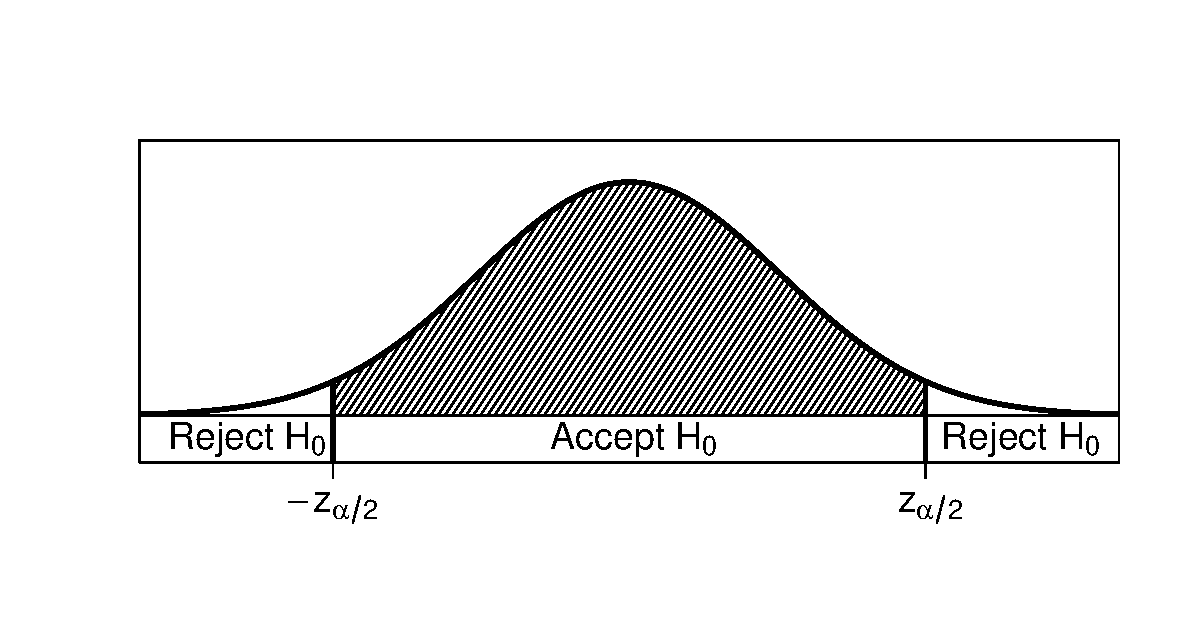
\includegraphics[width=0.98\textwidth, trim = 1.5cm 1.6cm 0.7cm 1.5cm, clip]{AcceptRegion}
\end{center}
\begin{itemize}\itemsep0.2cm
\item Significance level $\alpha$ $\Rightarrow$ each tail contains probability $\alpha/2$.
\item {\bf Acceptance region} lies within $\pm z_{\,\alpha/2}$.
\item {\bf Rejection region} lies outside of $\pm z_{\,\alpha/2}$.\\[0.3cm]
\end{itemize}
Note: If $n$ is small use  $\pm t_{\,\nu,\,\alpha/2}$ instead of $\pm z_{\,\alpha/2}$.
\end{frame}



\subsection{Proof Vs Evidence}
\begin{frame}{\bf \tcb{Proof Vs Evidence}}

Note that we {\bf never} use the word \emph{proof} since there is always some probability of error.\\[0.3cm]
\begin{itemize}\itemsep0.5cm
\item \emph{Cannot:}\,\, prove $H_0$ to be true or untrue.
\item \emph{Can:}\,\, provide evidence that $H_0$ is reasonable or unreasonable.\\[0.9cm]
\end{itemize}


If the test statistic falls into the {\bf acceptance region}, we say that the \emph{evidence against} $H_0$ is {\bf non-significant} $\Rightarrow$ we accept it.\\[0.6cm]


If the test statistic falls into the {\bf rejection region}, we say that the \emph{evidence against} $H_0$ is {\bf significant} $\Rightarrow$ we reject it.

\end{frame}



\subsection{Example: Tubs of Butter}
\begin{frame}{\bf \tcb{Example: Tubs of Butter}}

A machine is programmed to put 250g of butter into each tub. We wish to test this hypothesis at the 5\% level. Thus,\\[-0.2cm]
\begin{align*}
H_0: \quad \mu &= 250,\\
H_a: \quad \mu &\ne 250,\\[-0.2cm]
\end{align*}
i.e., the hypothesised value is $\mu_0 = 250$.\\[0.8cm]

We are testing at the 5\% level $\Rightarrow$ $\alpha = 0.05$ $\Rightarrow$ $\alpha/2 = 0.025$.\\[0.8cm]

Therefore, the critical values will be $\pm z_{\,0.025} = \pm 1.96$ or, if the selected sample is small, $\pm t_{\,\nu,\,0.025}$ where $\nu = n - 1$.

\end{frame}


\subsection{Example: Tubs of Butter}
\begin{frame}{\bf \tcb{Example: Tubs of Butter}}

We randomly select 35 tubs of butter and measure the contents. The average for this sample is 251.6g and the standard deviation is 3.1g.\\[0.6cm]

Since $n > 30$ the critical values are $\pm 1.96$.\\[0.6cm]

The test statistic is:
\begin{align*}
z =  \frac{\bar x - \mu_0}{\frac{s}{\sqrt{n}}} = \frac{251.6 - 250}{\frac{3.1}{\sqrt{35}}} = \frac{1.6}{0.524} = 3.05.\\
\end{align*}
The calculated $z = 3.05$ lies outside of $\pm 1.96$. Therefore we reject the null hypothesis that $\mu = 250$ at 5\% level of significance.\\[0.4cm]

Conclusion: the evidence suggests that the machine is \emph{not} working as programmed.


\end{frame}




\subsection{Question 1}
\begin{frame}{\bf \tcb{Question 1}}

A particular CPU design is expected to have a clock speed of 2.5Ghz. To test this hypothesis, 4 CPUs were selected and the results are as follows:
\begin{center}
\begin{tabular}{|cccc|}
\hline
&&&\\[-0.4cm]
2.53 & 2.55 & 2.54 & 2.24 \\[0.1cm]
\hline
\end{tabular}
\end{center}

\begin{enumerate}[a)]\itemsep0.2cm
\item State the null and alternative hypotheses.
\item What are the critical values (use $\alpha = 0.1$).
\item Calculate $\bar x$ and $s$.
\item Calculate the test statistic.
\item State your conclusion.
\end{enumerate}

\end{frame}





\section{Direction of Test}
\subsection{Two-Tailed Test}
\begin{frame}{\bf \tcb{Two-Tailed Test}}

For the butter tub example note that the alternative hypothesis was\\[-0.2cm]
\begin{align*}
H_a: \quad \mu \ne 250.\\[-0.4cm]
\end{align*}
If $\mu$ is \emph{not equal} to 250 $\Rightarrow$ it is either \emph{less than} 250 or \emph{greater than} 250:\\[-0.2cm]
\begin{align*}
\Rightarrow \quad H_a: \quad \mu < 250 \quad\text{or}\quad \mu > 250.\\[-0.4cm]
\end{align*}
{\bf The alternative hypothesis points to the rejection region}, i.e., we see that the rejection region appears in both the \emph{lower and upper tails} via the ``$<$'' and ``$>$'' inequality signs.\\[0.7cm]

Hence, this is known as a {\bf two-tailed} hypothesis test.

\end{frame}



\subsection{Two-Tailed Test}
\begin{frame}{\bf \tcb{Two-Tailed Test}}
%\begin{textblock}{3}(11.2,1.3)
%
\includegraphics[width=1\textwidth, trim = 0cm 0cm 0cm 0cm, clip]{Tails}
%\end{textblock}
\begin{center}
\begin{tabular}{|c@{\,\,}c|}
\hline
&\\[-0.4cm]
$H_0: \quad \mu$ & $= \mu_0$ \\[0.2cm]
$H_a: \quad \mu$ &  $\ne \mu_0$ \\[0.1cm]
\hline
\end{tabular}
\end{center}
\begin{center}
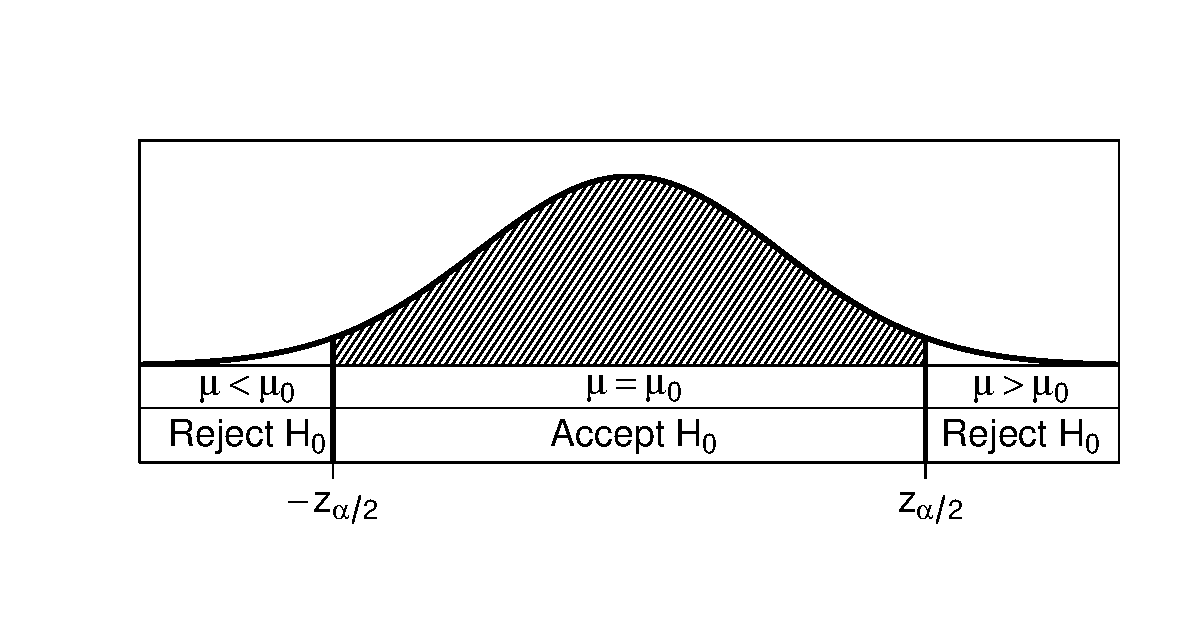
\includegraphics[width=0.98\textwidth, trim = 1.5cm 1.6cm 0.7cm 1.5cm, clip]{AcceptRegionTwo}
\end{center}
Note: If $n$ is small use  $\pm t_{\,\nu,\,\alpha/2}$ instead of $\pm z_{\,\alpha/2}$.
\end{frame}



\subsection{One-Tailed Test}
\begin{frame}{\bf \tcb{One-Tailed Test}}

In other situations, it makes more sense to carry out a {\bf one-tailed} test.\\[0.4cm]

Consider the gameplay example. Really it is of interest to test the null hypothesis that there are \emph{at least} 16 hours of gameplay:\\[-0.2cm]
\begin{align*}
H_0: \quad \mu \ge 16.\\[-0.3cm]
\end{align*}
Thus, the alternative hypothesis is\\[-0.2cm]
\begin{align*}
H_a: \quad \mu < 16.\\[-0.3cm]
\end{align*}

For a one-tailed test we {\bf do not divide} \boldmath$\alpha$ {\bf by two} since all of this probability goes into \emph{one} tail.\\[0.4cm]

{\bf The alternative hypothesis points to the rejection region}.

\end{frame}


\subsection{One-Tailed Test: Lower Tail}
\begin{frame}{\bf \tcb{One-Tailed Test: Lower Tail}}
\begin{center}
\begin{tabular}{|c@{\,\,}c|}
\hline
&\\[-0.4cm]
$H_0: \quad \mu$ & $\ge \mu_0$ \\[0.2cm]
$H_a: \quad \mu$ &  $< \mu_0$ \\[0.1cm]
\hline
\end{tabular}
\end{center}
\begin{center}
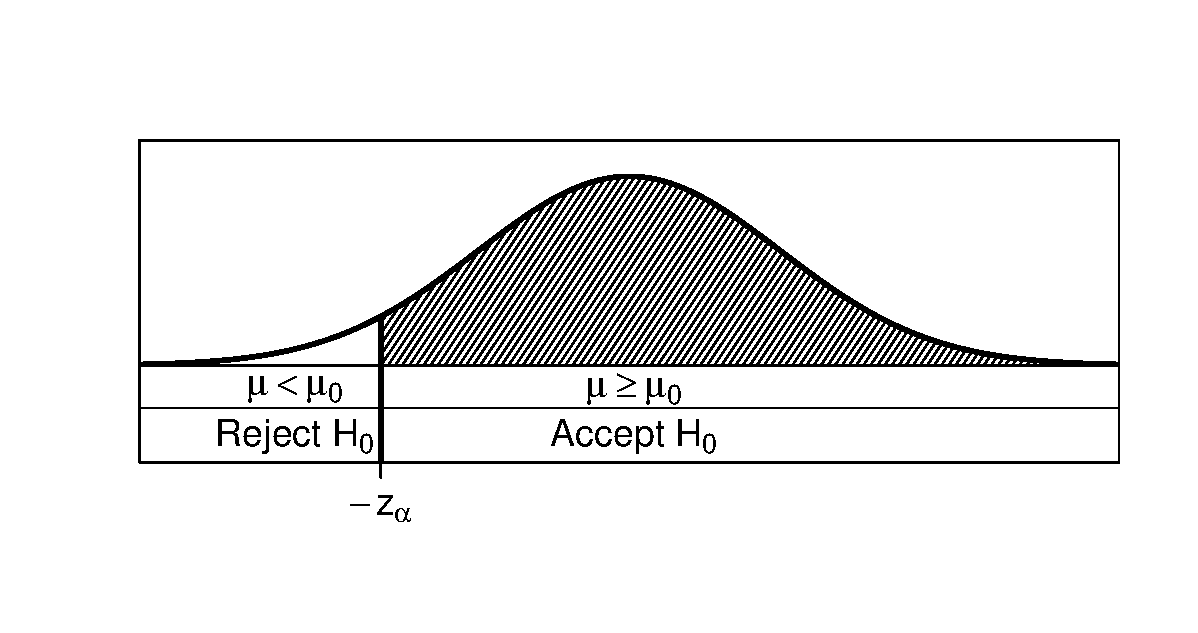
\includegraphics[width=0.98\textwidth, trim = 1.5cm 1.6cm 0.7cm 1.5cm, clip]{AcceptRegionOne1}
\end{center}
Note: If $n$ is small use  $- t_{\,\nu,\,\alpha}$ instead of $- z_{\,\alpha}$.
\end{frame}

\subsection{One-Tailed Test: Upper Tail}
\begin{frame}{\bf \tcb{One-Tailed Test: Upper Tail}}
\begin{center}
\begin{tabular}{|c@{\,\,}c|}
\hline
&\\[-0.4cm]
$H_0: \quad \mu$ & $\le \mu_0$ \\[0.2cm]
$H_a: \quad \mu$ &  $> \mu_0$ \\[0.1cm]
\hline
\end{tabular}
\end{center}
\begin{center}
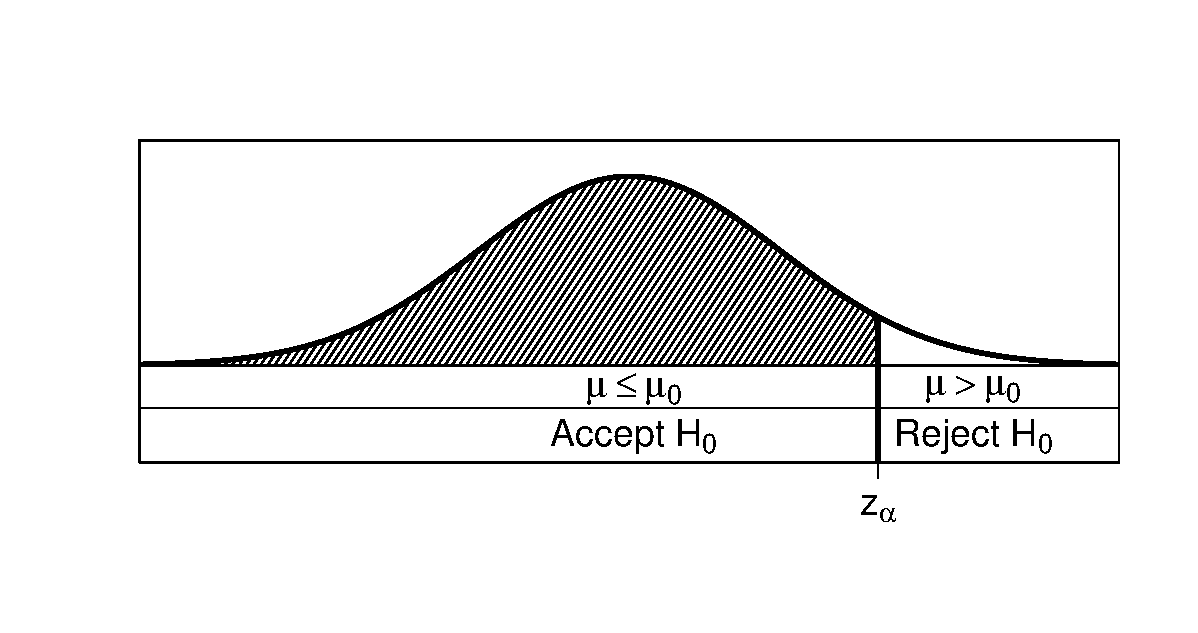
\includegraphics[width=0.98\textwidth, trim = 1.5cm 1.6cm 0.7cm 1.5cm, clip]{AcceptRegionOne2}
\end{center}
Note: If $n$ is small use  $t_{\,\nu,\,\alpha}$ instead of $ z_{\,\alpha}$.
\end{frame}



\subsection{Direction of Test}
\begin{frame}{\bf \tcb{Direction of Test}}

\begin{center}
\begin{tabular}{|c@{\,\,}c|c|c|c|}
\hline
&&&&\\[-0.2cm]
\multicolumn{2}{|c|}{Hypotheses}  & Tails & Critical Values & Rejection Region\\[0.2cm]
\hline
&&&&\\[-0.2cm]
$H_0: \quad \mu$ & $= \mu_0$   & \multirow{2}{*}{Two} & \multirow{2}{*}{$\pm z_{\,\alpha/2}$\,\, or \,\,$\pm t_{\,\nu,\,\alpha/2}$} & \multirow{2}{*}{Outside critical values}  \\[0.2cm]
$H_a: \quad \mu$ &  $\ne \mu_0$ &&& \\[0.3cm]
\hline
&&&&\\[-0.2cm]
$H_0: \quad \mu$ & $\ge \mu_0$  & \multirow{2}{*}{One} & \multirow{2}{*}{$- z_{\,\alpha}$\,\, or \,\,$- t_{\,\nu,\,\alpha}$} & \multirow{2}{*}{Below critical value}   \\[0.2cm]
$H_a: \quad \mu$ &  $< \mu_0$ &&&\\[0.3cm]
\hline
&&&&\\[-0.2cm]
$H_0: \quad \mu$ & $\le \mu_0$ & \multirow{2}{*}{One} & \multirow{2}{*}{$ z_{\,\alpha}$\,\, or \,\,$ t_{\,\nu,\,\alpha}$} & \multirow{2}{*}{Above  critical value}  \\[0.2cm]
$H_a: \quad \mu$ &  $> \mu_0$ &&& \\[0.3cm]
\hline
\end{tabular}
\end{center}

Note: the null hypothesis {\bf always} contains the equals.

\end{frame}


\subsection{Example: Gameplay}
\begin{frame}{\bf \tcb{Example: Gameplay}}

We return to the gameplay example.\\[0.4cm]

A games developer wishes to test the null hypothesis that their game has \emph{at least} 16 hours of gameplay using the 5\% level of significance.\\[0.4cm]

Thus the hypotheses are:
\begin{align*}
H_0: \quad \mu &\ge 16\\[0.2cm]
H_a: \quad \mu &< 16\\[-1cm]
\end{align*}
\begin{itemize}\itemsep0.4cm
\item One-sided test $\Rightarrow$ use $\alpha = 0.05$ (do \emph{not} divide by two).
\item Alternative hypothesis points to the \emph{lower tail} $\Rightarrow$ $- z_{\,\alpha}$\,\, or \,\,$- t_{\,\nu,\,\alpha}$.
\end{itemize}

\end{frame}



\subsection{Example: Gameplay}
\begin{frame}{\bf \tcb{Example: Gameplay}}

From a sample of $n= 33$, $\bar x = 15.4$ and $s = 2.3$.\\[0.4cm]

Note that $n >30$ $\Rightarrow$ the critical value is $- z_{\,0.05} = -1.64$.\\[0.4cm]

The test statistic is:\\[-0.2cm]
\begin{align*}
z =  \frac{\bar x - \mu_0}{\frac{s}{\sqrt{n}}} = \frac{15.4 - 16}{\frac{2.3}{\sqrt{33}}} = \frac{-0.6}{0.4} = -1.5.\\[-0.3cm]
\end{align*}
Since $z=-1.5$ is \emph{not} in the rejection region (i.e., the region below $-1.64$), we accept $H_0: \mu \ge 16$ at the 5\% level.\\[0.6cm]

Conclusion: the number of gameplay hours is sufficient (at least 16) and, therefore, we do not have to add extra content to the game.

\end{frame}



\subsection{Question 2}
\begin{frame}{\bf \tcb{Question 2}}
Assume that a particular CPU is designed to have a normal operating temperature of 30 degrees or less. A sample of 40 CPUs were tested: the average for this sample was 32 degrees and the variance was 10 degrees-squared.\\[0.5cm]

We wish to test the hypothesis that the temperature is less than or equal to 30 degrees at the 1\% level.\\[0.2cm]
\begin{enumerate}[a)]\itemsep0.3cm
\item State the null and alternative hypotheses.
\item Define the rejection region.
\item Calculate the test statistic.
\item State your conclusion.
\end{enumerate}

\end{frame}





\section{Errors}
\subsection{Decisions}
\begin{frame}{\bf \tcb{Decisions}}

When we carry out a hypothesis test, there are two possible decisions:\\[0.1cm]
\begin{enumerate}[a)]\itemsep0.3cm
\item Reject $H_0$.
\item Accept $H_0$.\\[0.8cm]
\end{enumerate}

This leads to four different scenarios:\\[0.1cm]
\begin{enumerate}[i)]\itemsep0.3cm
\item Reject $H_0$ when $H_0$ is true $\Rightarrow$ {\bf type 1 error}.
\item Reject $H_0$ when $H_0$ is false.
\item Accept $H_0$ when $H_0$ is true.
\item Accept $H_0$ when $H_0$ is false  $\Rightarrow$  {\bf type 2 error}.
\end{enumerate}


\end{frame}


\subsection{Errors}
\begin{frame}{\bf \tcb{Errors}}

We fix the probability of wrongly \emph{rejecting} $H_0$ at the $\alpha$ level:\\[-0.2cm]
\begin{align*}
\Pr(\text{Reject } H_0 \,\,|\,\, H_0 \text{ is true}) = \alpha,\\[-0.2cm]
\end{align*}
i.e., we control the probability of a {\bf type 1 error}.\\[1cm]

The probability of wrongly \emph{accepting} $H_0$ is\\[-0.2cm]
\begin{align*}
\Pr(\text{Accept } H_0 \,\,|\,\, H_0 \text{ is false}) = \beta,\\[-0.2cm]
\end{align*}
i.e., a {\bf type 2 error}.

\end{frame}


\subsection{Relationship Between $\alpha$ and $\beta$}
\begin{frame}{\bf \tcb{Relationship Between $\alpha$ and $\beta$}}

The value of $\beta$ {\bf depends on} $\alpha$. It can be \emph{calculated} once we have chosen the $\alpha$ level.\\[0.8cm]

We will not calculate $\beta$ in this course but just know the relationship:\\[0.5cm]
\begin{center}
{\bf Decreasing {\boldmath$\alpha$} leads to an increase in {\boldmath$\beta$}}.\\[0.5cm]
\end{center}

If we reduce $\alpha$, the acceptance region increases $\Rightarrow$ rejection of $H_0$ is less likely $\Rightarrow$ we are more open to a type 2 error.\\[0.8cm]

In practice, these values will be chosen to reflect the costs (often monetary) associated with making the two types of error.

\end{frame}














\section{P Value}
\subsection{Example: Tubs of Butter}
\begin{frame}{\bf \tcb{Example: Tubs of Butter}}

Recall that in the butter tub example we had the following hypotheses:
\begin{align*}
H_0: \quad \mu &= 250\\
H_a: \quad \mu &\ne 250\\[-0.3cm]
\end{align*}

We tested $H_0$ at the 5\% level and, since the test is two-tailed and $n$ was large, the critical values were $z_{\,0.025} = \pm 1.96$.\\[0.6cm]


The test statistic $z = 3.05$ and, since this is outside of $\pm 1.96$, we rejected $H_0$ at the 5\% level.\\[0.6cm]

However, with $z=3.05$, the evidence is stronger than the 5\% level. In fact we would reject $H_0$ at the 1\% level also (since $z_{\,0.005} = \pm 2.58$).

\end{frame}


\subsection{Example: Tubs of Butter}
\begin{frame}{\bf \tcb{Example: Tubs of Butter}}

The question that arises is, just how strong is the evidence against $H_0$?\\[0.9cm]

What is the lowest $\alpha$ level at which we would reject $H_0$ if $z=3.05$? We require the $\alpha$ level that leads to the critical values $z_{\,\alpha/2} = \pm 3.05$.\\[0.9cm]

From the normal tables we find that $\Pr(Z > 3.05) = 0.00114$. This is the $\alpha/2$ value $\Rightarrow$ $\alpha = 2(0.00114) = 0.00228$ is the lowest $\alpha$ level at which $H_0$ would be rejected.\\[0.9cm]

Thus, we can see that the evidence against $H_0$ is very strong.

\end{frame}



\subsection{P-Value}
\begin{frame}{\bf \tcb{P-Value}}

The quantity we have just calculated is called a {\bf p-value}.\\[0.4cm]

It tells us the how likely the data is if $H_0$ were true. Thus, a p-value is a measure of {\bf evidence against} {\boldmath$H_0$}:\\[0.2cm]
\begin{itemize}\itemsep0.3cm
\item Small p-value $\Rightarrow$ data is unlikely under $H_0$ $\Rightarrow$ evidence to reject $H_0$.
\item Large p-value $\Rightarrow$ data is likely under $H_0$ $\Rightarrow$ evidence to accept $H_0$.\\[0.5cm]
\end{itemize}

We can calculate p-values as follows:
\begin{align*}
\boxed{\text{p-value } = \left\{
\begin{array}{rl}
2 \times \Pr(Z > |z|) & \text{if }  H_a: \, \mu \ne \mu_0\\[0.2cm]
\Pr(Z < z) & \text{if } H_a: \, \mu < \mu_0\\[0.2cm]
\Pr(Z > z) & \text{if } H_a: \, \mu > \mu_0\\
\end{array} \right.}
\end{align*}

{\footnotesize(note: $|z|$ is the \emph{absolute value} of $z$)}

\end{frame}




\subsection{P-Value}
\begin{frame}{\bf \tcb{P-Value}}

Since 1\%, 5\% and 10\% are commonly used significance levels, we can use the following as a rough guide to interpreting p-values:\\[0.3cm]

\begin{itemize}\itemsep0.6cm
\item $0.00 <$ p-value $< 0.01$ $\Rightarrow$ strong evidence against $H_0$.
\item $0.01 <$ p-value $< 0.05$ $\Rightarrow$  evidence against $H_0$.
\item $0.05 <$ p-value $< 0.10$ $\Rightarrow$  some evidence against $H_0$ (not strong).
\item $0.10 <$ p-value $< 1.00$ $\Rightarrow$  no evidence against $H_0$.
\end{itemize}


\end{frame}





\subsection{Example: Gameplay}
\begin{frame}{\bf \tcb{Example: Gameplay}}

Recall that in the gameplay example:
\begin{align*}
H_0: \quad \mu &\ge 16\\[0.2cm]
H_a: \quad \mu &< 16\\[-0.5cm]
\end{align*}

This is a one-sided test (with rejection region in the lower tail) and, therefore, the p-value is $\Pr(Z < z)$ where $z$ is the test statistic.\\[0.4cm]

Since the calculated test statistic was $z=-1.5$, we have
\begin{align*}
\text{p-value } = \Pr(Z < -1.5) = \Pr(Z > 1.5) = 0.0668.
\end{align*}

Thus, although there is some evidence against $H_0$, it is not strong.\\[0.4cm] Furthermore,  since the stated significance level was $\alpha = 0.05$ in this example, we would not reject $H_0$.

\end{frame}





\section{Proportions}
\subsection{Proportions}
\begin{frame}{\bf \tcb{Other Parameters}}


We have introduced the idea of hypothesis testing using $\mu$.\\[0.8cm]

The general procedure is much the same for other parameters.\\[0.8cm]

That is, we calculate:\\
\begin{align*}
z = \frac{\text{statistic }-\text{ hypothesised value}}{\text{standard error}}\\
\end{align*}
and then compare this to a critical value.


\end{frame}



\subsection{Proportions}
\begin{frame}{\bf \tcb{Proportions}}

Recall that for a proportion, the \emph{true} standard error is $\sigma(\,\widehat{\!P}) = \sqrt{\frac{p\,(1-p)}{n}}$.\\[0.8cm]

For the calculation of confidence intervals, we replaced $p$ with $\hat p$ (since $p$ is unknown) $\Rightarrow$ $s(\,\widehat{\!P}) = \sqrt{\frac{\hat p\,(1-\hat p)}{n}}$. \\[0.8cm]

For hypothesis testing, we use the {\bf hypothesised value} $p = p_0$:\\
\begin{align*}
\boxed{s(\,\widehat{\!P}) = \sqrt{\frac{p_0\,(1-p_0)}{n}}}.\\[-0.4cm]
\end{align*}

Apart from this difference, everything is the same as in the case of hypothesis testing for $\mu$ as covered already.

\end{frame}



\subsection{Example: User Age}
\begin{frame}{\bf \tcb{Example: User Age}}

A company believes that 70\% of users of their product are teenagers; this impacts advertising campaigns. They wish to test this hypothesis. Therefore, we have the following null and alternative hypotheses:\\[-0.2cm]
\begin{align*}
H_0: \quad p &= 0.7\\[0.2cm]
H_a: \quad p &\ne 0.7\\[-0.5cm]
\end{align*}

A random sample of users were selected and it was found that 40 out of 75 were teenagers, i.e., $\hat p = \frac{40}{75} = 0.533$.

\begin{align*}
\Rightarrow z = \frac{\hat p - p_0}{\sqrt{\frac{p_0\,(1-p_0)}{n}}} = \frac{0.533 - 0.7}{\sqrt{\frac{0.7\,(0.3)}{75}}} = \frac{-0.167}{0.0529} = -3.16.
\end{align*}

{\bf Note that {\boldmath$p_0$} is used in the standard error}.


\end{frame}



\subsection{Example: User Age}
\begin{frame}{\bf \tcb{Example: User Age}}

We will view the evidence against $H_0$ using the p-value approach. Since this is a two tailed test we have:

\begin{align*}
\text{p-value} = 2 \, \Pr(Z > |z|) &= 2 \, \Pr(Z > |-3.16|) \\[0.1cm]
&= 2 \, \Pr(Z > 3.16) \\[0.1cm]
&= 2 \, (0.00079) \\[0.1cm]
&= 0.00158. \\[0.1cm]
\end{align*}

Thus, it appears that $H_0$ is unlikely. The proportion of teenagers who use the product is not as much as they thought.


\end{frame}



\subsection{Question 3}
\begin{frame}{\bf \tcb{Question 3}}

A new version of an operating system is being developed. A beta version is released to some randomly selected individuals who are then asked: ``Do you prefer the new system?''.\\[0.2cm]

By default, the company will assume that the old system is preferred, i.e., the hypothesis to be tested is $p \le 0.5$.\\[0.2cm]

It was found that 38 out of 65 people prefer the new system.\\[0.3cm]

\begin{enumerate}[a)]\itemsep0.2cm
\item State the null and alternative hypotheses.
\item What is the critical value if $\alpha = 0.05$?
\item Calculate the test statistic.
\item Provide your conclusion.
\item Calculate a p-value also.
\end{enumerate}


\end{frame}





\end{document} 